A topologia sempre foi vista como uma área de abstração da matemática, sem
espaço para aplicações. Ela é usada para o estudo de diversos espaços
em sua forma abstrata, auxiliando matemáticos em diversas demonstrações
de teoremas e dando uma base fundamental para grande parte da teoria matemática
usada no dia a dia~\cite{Poincare1895}.

Certas propriedades dos espaços topológicos são estudadas através da
topologia algébrica, dando algumas informações, como o número de componentes
conexas por caminhos de um espaço e buracos. A princípio esta é uma área altamente
abstrata da matemática,  nos últimos anos esta visão foi mudando,
com o desenvolvimento da Homologia Persistente e Análise Topológica de Dados.

Um conjunto de dados, geralmente um subconjunto finito de algum espaço métrico,
pode ser estudado através da homologia persistente e assim obtemos informações
topológicas do objeto em estudo.

O pipeline da análise topológica de dados pode ser divido nos seguintes passos:
\begin{itemize}
  \item A entrada do algoritmo pode ser um conjunto de pontos ou alguma matriz
  de distância/similaridade do conjunto de dados.
  \item A construção de um objeto combinatorial em cima do conjunto de dados ou
  da matriz de distância. Geralmente uma filtração ou um complexo simplicial.
  \item A partir da filtração ou do complexo simplicial é possível extrair informações
  topológicas e geométricas do conjunto de dados, por exemplo o número de
  componentes conexas, como um algoritmo de Clustering.
  \item Por fim a interpretação dos dados obtidos e possível pós processamento
  para a utilização em outros algoritmos, como os de classificação ou regressão.
\end{itemize}

Neste capítulo descrevemos de forma ingênua a homologia persistente, começando com
filtrações, passando pelos espaços vetoriais associados
aos complexos simpliciais e chegando ao algoritmo de homologia persistente.
Mostraremos também como interpretar os resultados obtidos.
A~\autoref{fig:pipeline_hp} mostra os passos para utilizar esta ferramenta em um conjunto de dados.

\begin{figure}
  \centering
  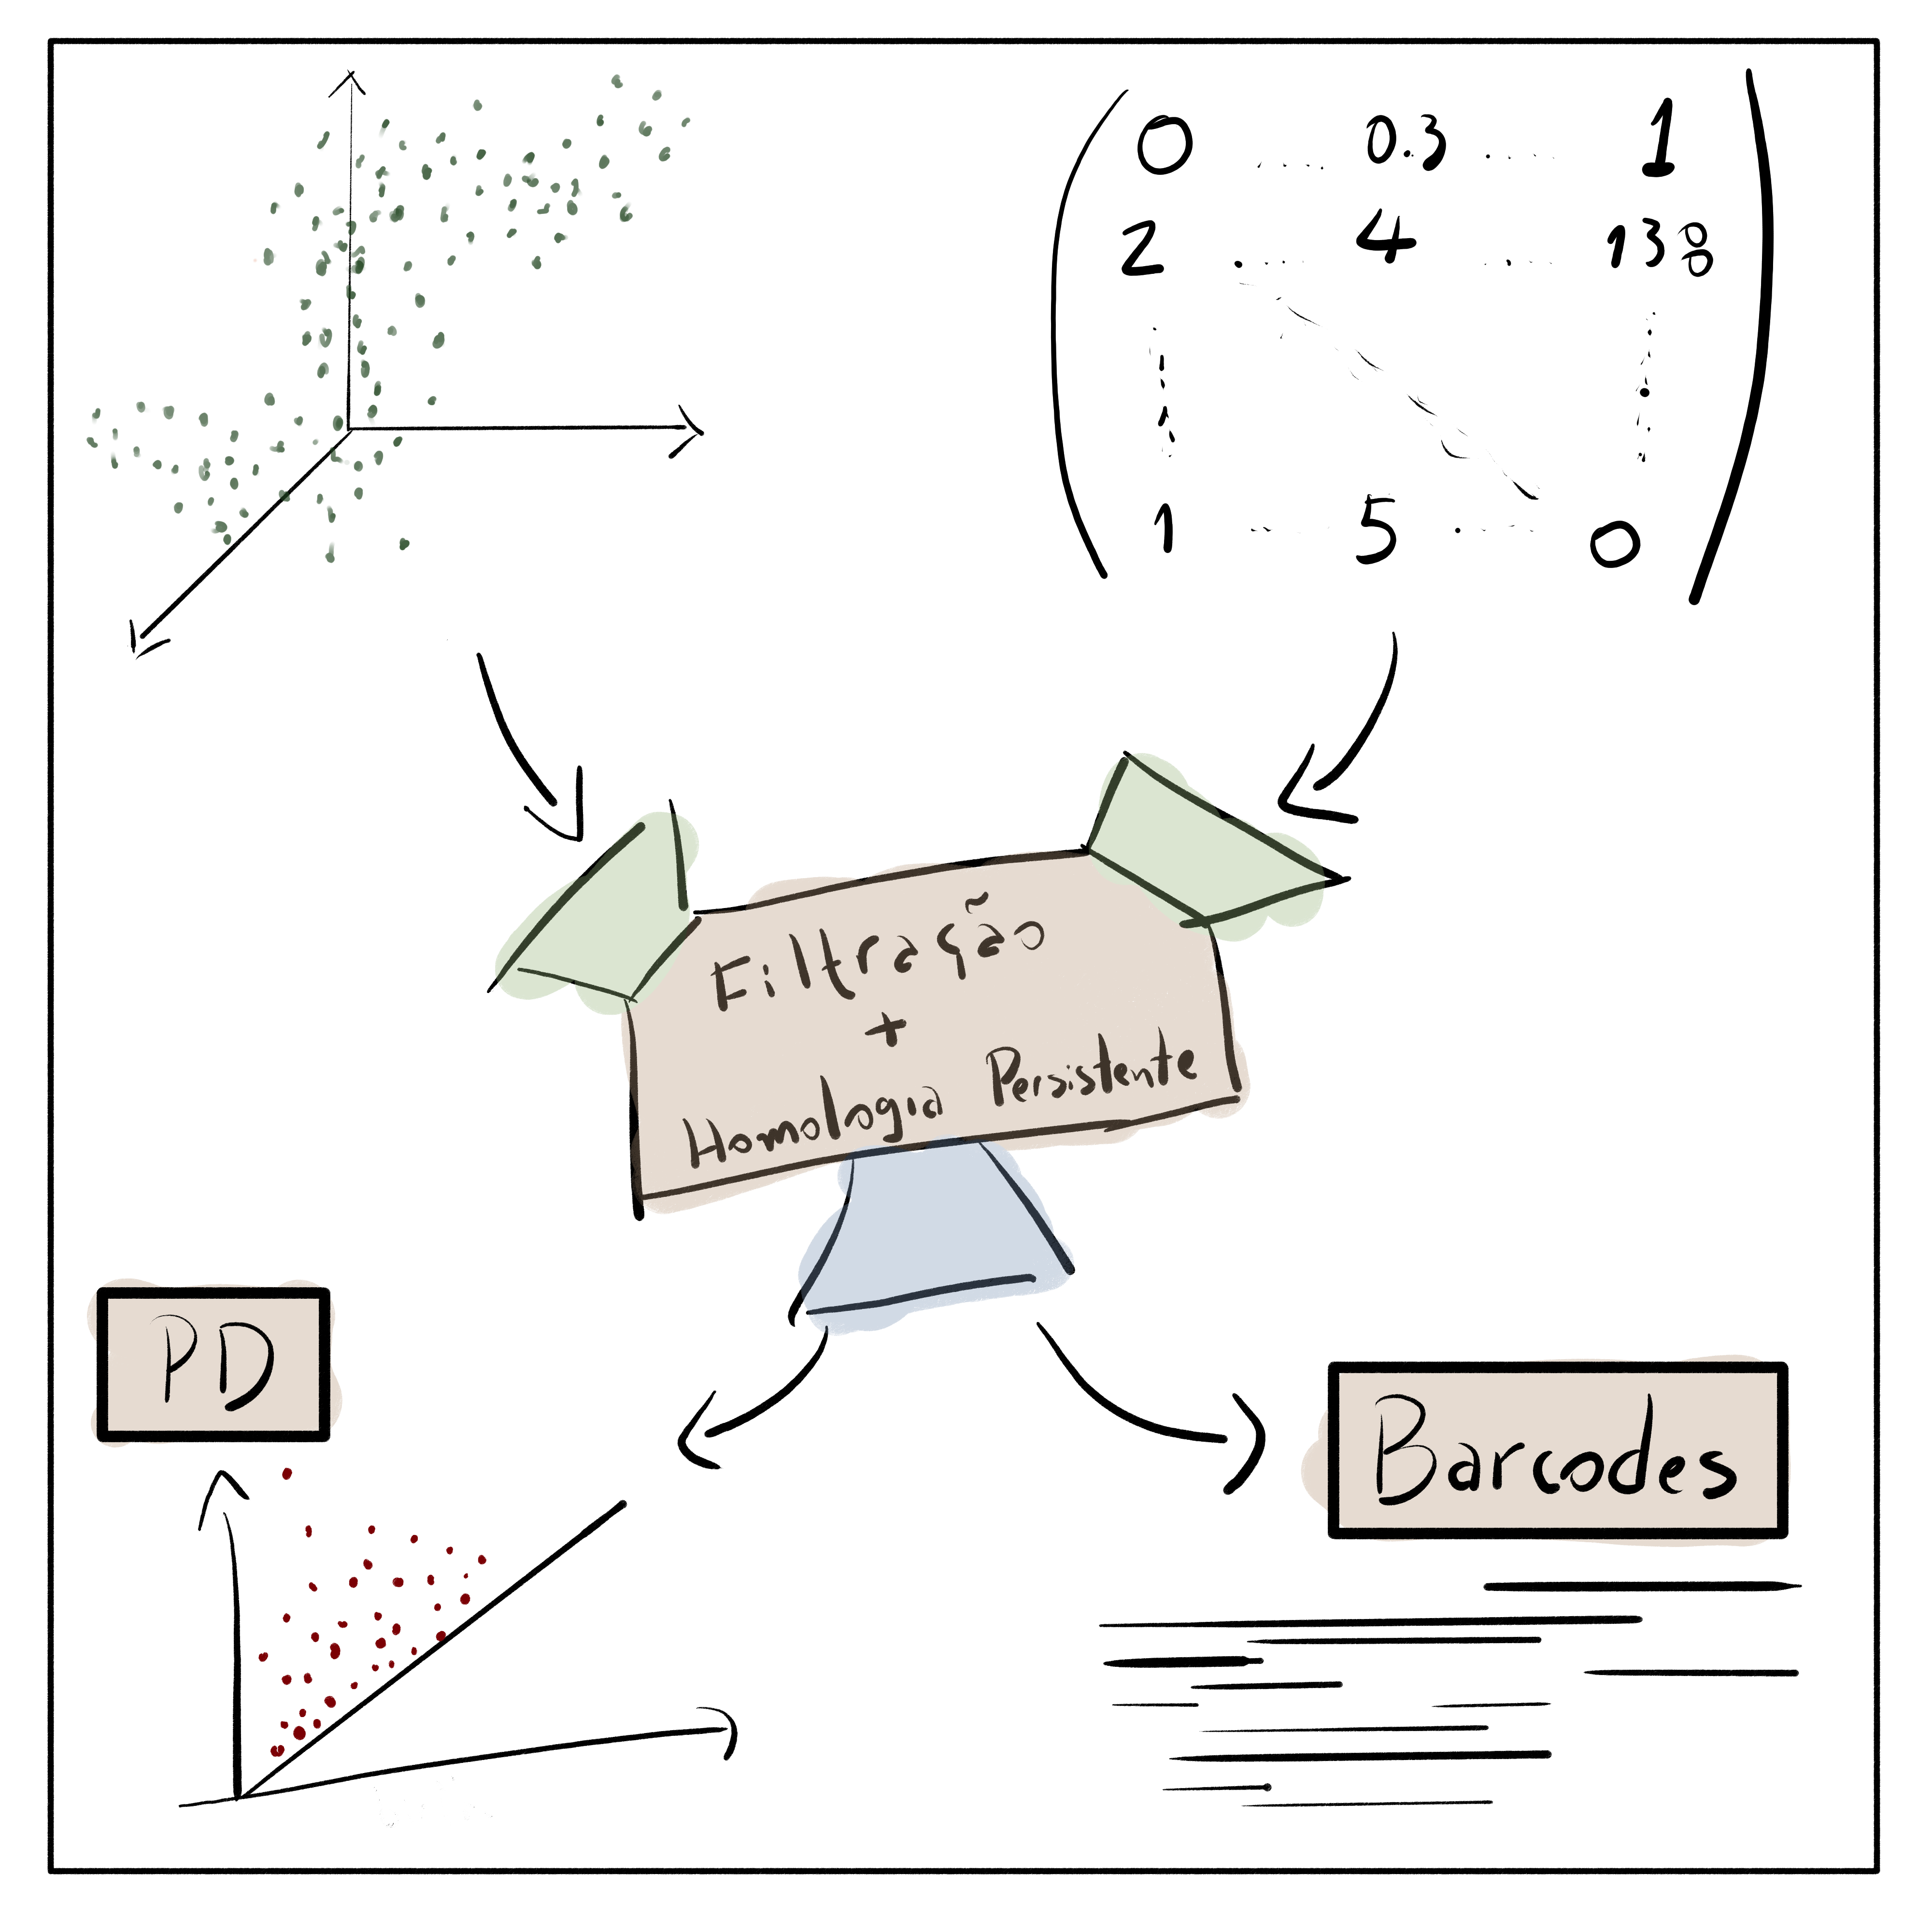
\includegraphics[width=0.7\textwidth]{images/pipeline_hp.png}
  \caption{Representação do pipeline para a utilização da homologia persistente
          com um conjunto de dados.}
  \label{fig:pipeline_hp}
\end{figure}


\section{Filtrações}
A filtração de um conjunto de dados é o primeiro passo na nossa sequência apresentada
na~\autoref{fig:pipeline_hp}.
Dado um conjunto de dados precisamos construir um objeto combinatorial de forma
que possa ser analisado do ponto de vista da topologia assim como computacionalmente.
A filtração é este objeto que captura as mudanças do conjunto dada uma escala.

Algumas definições se fazem necessárias para entendermos o que é a filtração
e qual o seu papel na análise topológica de dados. Começamos definindo um simplexo,
primeiro objeto combinatorial que é a base da filtração.

\begin{defi}
  Sejam $v_0, v_1, \dots, v_k \in \mathbb{R}^n$ linearmente afins, ou seja $\{v_1 - v_0, \dots, v_k - v_0\}$
  é um conjunto linearmente independente. O k-simplexo definido pelos pontos acima,
  chamados de vértices, é o conjunto

  \begin{equation*}
    \Set{\sum_{i=0}^k \lambda_i v_i \ | \ \sum_{i=0}^k \lambda_i = 1 \text{ e }
          \lambda_i \ge 0, \ \forall i}.
  \end{equation*}
\end{defi}

Note que para $k = 0$, temos um único vértice. Para $k=1$, temos uma reta, já
para $k=2$ temos um triângulo preenchido. E no caso $k=3$, um tetraedro. Os
simplexos podem ser vistos na~\autoref{fig:ksimpl}. Além disso, dizemos que a dimensão
do $k$-simplexo é $k$. A envoltoria convexa de qualquer subconjunto dos vértices
de um simplexo $S$ é chamado de face de $S$.

\begin{figure}
  \centering
  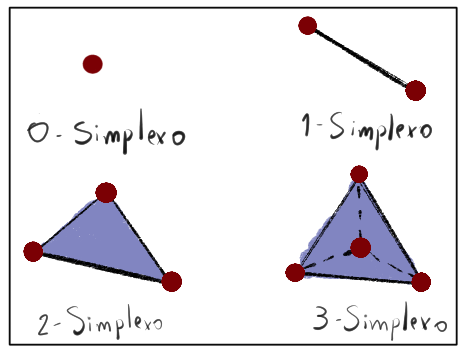
\includegraphics[width=0.7\textwidth]{images/ksimpl.png}
  \caption{Exemplos de $k$-simplexos para $k\in \Set{0,1,2,3}$.}
  \label{fig:ksimpl}
\end{figure}

Tendo definido os $k$-simplexos, podemos definir o complexo simplicial.
\begin{defi}
    Um complexo simplicial $K$ é uma coleção de simplexos satisfazendo as seguintes
    relações:
    \begin{itemize}
      \item Dado $\sigma \in K$, temos que para toda face $\tau \subset \sigma$
            vale $\tau \in K$.
      \item A interseção de dois simplexos é face de ambos os simplexos, em outras palavras,
      $\sigma, \tau \in K$ implica que $\sigma \cap \tau \subset \sigma$ e
      $\sigma \cap \tau \subset \tau$.
    \end{itemize}
\end{defi}
A segunda condição é necessária para evitar casos patológicos como mostrado na
\autoref{fig:simp_path}. Dizemos que a dimensão do complexo simplicial $K$ é a maior dimensão dentre os
simplexos em $K$. Podemos definir agora a filtração de um complexo simplicial.


\begin{figure}
  \centering
  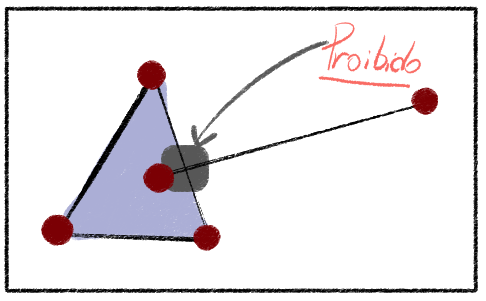
\includegraphics[width=0.7\textwidth]{images/simp_path.png}
  \caption{Exemplo em que a interseção de dois simplexos não é um simplexo.}
  \label{fig:simp_path}
\end{figure}

\begin{defi}
  Seja $K$ um complexo simplicial. Definimos uma filtração de $K$ sendo uma
  sequência de subconjuntos $K_i \subset K$, com $i \in \{ 1, \dots, n \}$,
  de tal forma que $K_i$ é um complexo simplicial para todo $i$ e vale que
  \begin{equation*}
    K_1 \subset \dots \subset K_{n-1} \subset K_n = K.
  \end{equation*}
\end{defi}
Na~\autoref{fig:filtracao_exemplo} temos um exemplo de filtração para um complexo
simplicial.

\begin{figure}[hbt]
  \centering
  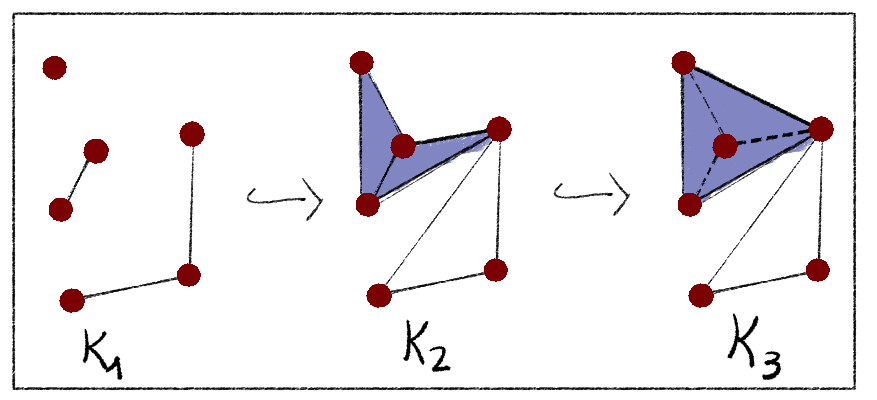
\includegraphics[width=0.7\textwidth]{images/filtracao_exemplo.png}
  \caption{Exemplo de filtração para um complexo simplicial $K$.}
  \label{fig:filtracao_exemplo}
\end{figure}


\subsection{Filtração de Čech}

\subsection{Filtração de Vietoris-Rips}

\subsection{Filtração \textit{Alpha Shape}}

\section{A matriz de bordo $\partial$}

\section{Redução da matriz}
